\section{Eigenvalue solution by Power Method on GPU}
\label{sec:ev}
The last problem concerns the evaluation of eigenvalue using the power method via a paralellized CUDA code. Reference for this implementation is a sequantial CPU-code provided by the course (\texttt{power\_cpu.cu}).\\

A scematic overview of the iteration loop for the power method is shown bellow in algorithm \autoref{alg:power_method}. The whole implementation details can be found in the appendix for the current section.\\
\begin{algorithm}
    \caption{\Shining{GPU Power Method}}
    \label{alg:power_method}
    \begin{algorithmic}[1]
    \State \textbf{Input:} Matrix $\mathbf{A}$ of size $N \times N$, tolerance $\epsilon$, maximum iterations $max\_iter$
    \State \textbf{Output:} Dominant eigenvalue $\lambda$
    
    \State Initialize $\mathbf{v}$ with $v_1 = 1, v_i = 0$ for $i > 1$
    \State $\lambda_\text{Old} \gets 0$, $\lambda \gets 0$
    \State Allocate GPU memory for $\mathbf{A}$, $\mathbf{v}$, $\mathbf{w}$, and $\lambda$
    \State Copy $\mathbf{A}$ and $\mathbf{v}$ to GPU memory
    \State $\mathbf{w} \gets \mathbf{A} \cdot \mathbf{v}$ \Comment{First iteration of $\mathbf{w}$ computation using $\texttt{Av\_Product}$ kernel}
    
    \For{$i = 0$ to $max\_iter - 1$}
        \State Compute norm of $\mathbf{w}$: $\text{norm} \gets \sqrt{\mathbf{w}^T \cdot \mathbf{w}}$ \Comment{Using $\texttt{FindNormW}$ kernel}
        \State Normalize $\mathbf{v}$: $\mathbf{v} \gets \mathbf{w} / \text{norm}$ \Comment{Using $\texttt{NormalizeW}$ kernel}
        \State Compute $\mathbf{w} \gets \mathbf{A} \cdot \mathbf{v}$ \Comment{Using $\texttt{Av\_Product}$ kernel}
        \State Compute eigenvalue: $\lambda \gets \mathbf{v}^T \cdot \mathbf{w}$ \Comment{Using $\texttt{FindNormW}$ kernel}
        \If{$|\lambda - \lambda_\text{Old}| < \epsilon$}
            \State \textbf{Break} \Comment{Convergence achieved}
        \EndIf
        \State $\lambda_\text{Old} \gets \lambda$
    \EndFor
    
    \State Copy $\lambda$ back to host memory
    \State Deallocate GPU memory
    \end{algorithmic}
\end{algorithm}

\textbf{Note:} A $sqrt()$ was added in the \texttt{NormalizeW} kernel over \texttt{g\_NormW[0]}. This way we can use the output of \texttt{FindNormW} directly in the \texttt{NormalizeW} kernel.\\


I performed all the following measurements after throwing away the first GPU run (burner-run). The reason beaing, that the first run always took around 10 times longer than the following runs. This is likely due to some GPU initialization and setup overhead. It should also be noted, that I freed the GPU memory after each run to avoid caching effects. The basic setup in the main looks like this schematically: 
\lstinputlisting[language=c]{input/code/03/gpu_main.c}
Here \texttt{RunGPUPowerMethod} runs the power method on the GPU and on the top we can see the burner run. \texttt{CleanGPU} is a function that frees the allocated memory on the GPU as mentioned above.\\

\Shining{Iterations to convergence needed}\\
While performing the different measurements on the GPU it stood out to me, that the iterations needed to reach the specified tolerance ($\epsilon = 0.000005$) varied quite a bit. It was evident, that the GPU reaches a value very close to the eigenvalue rather fast (on the second iteration). However, the final convergence seems to depend on the precision of the operations. For the CPU we always perform the same operations in the same order, thus leading to the same results every time. The GPU on the other hand perfroms the calculations in parallel and especially for the accumulation operations the order of operations will certainly vary. Small rounding error introduced by the floating point percision in combination with a small $\epsilon$ can now lead to differences: These arise because the rounding in the accumulation functions such as \texttt{FindNormW} and \texttt{ComputeLamda} is dependant on the order of operations (not associative)! It should also be noted that the T4 GPUs used on Google Colab support only FP32 operations, thus moving to FP64 wasn't an option. \\

\textbf{All of the following benchmarks are perfromed in the supplied IPython notebook on Google Collab using T4 GPUs.}\\ 

\subsection{Step 1: Shared vs. global memory for matrix-vector multiplication}
As can be seen in the code snippet from above, we perfrom multiple runs of the power method on the GPU. First with global memory and then with shared memory. This is done by using different kernels for the AV-product. The kernel used for shared memory is unchanged.
Furthermore, to investigate the performance impact of shared vs. global memory during the matrix vector multiplication we first need an alternative kernel which doesn't use shared memory. This kernel is given bellow: 
\lstinputlisting[language=c]{input/code/03/Av_Product_Global.c}
Notice that the kernel above doesn't need to copy data from global to shared memory, this makes it possible to efficiently calculate the AV-product in a striped partitioning fashing. Furthermore, we do not need any syncronisation here in contrast to the original kernel. Given this, at least from a instruction flow perspective, one may think that the global memory kernel is heavily favoured due to it's simplicity. We shall see if this holds up given our measurements. \\ 
Subsequently, 10 measurements are perfromed with the original kernel and the changed kernel to determine the mean total runtimes depending on memory usage patterns. 
We obtain a \Shining{scatter plot} seen in \autoref{fig:cuda_step1}
\begin{figure}[H]
    \centering
    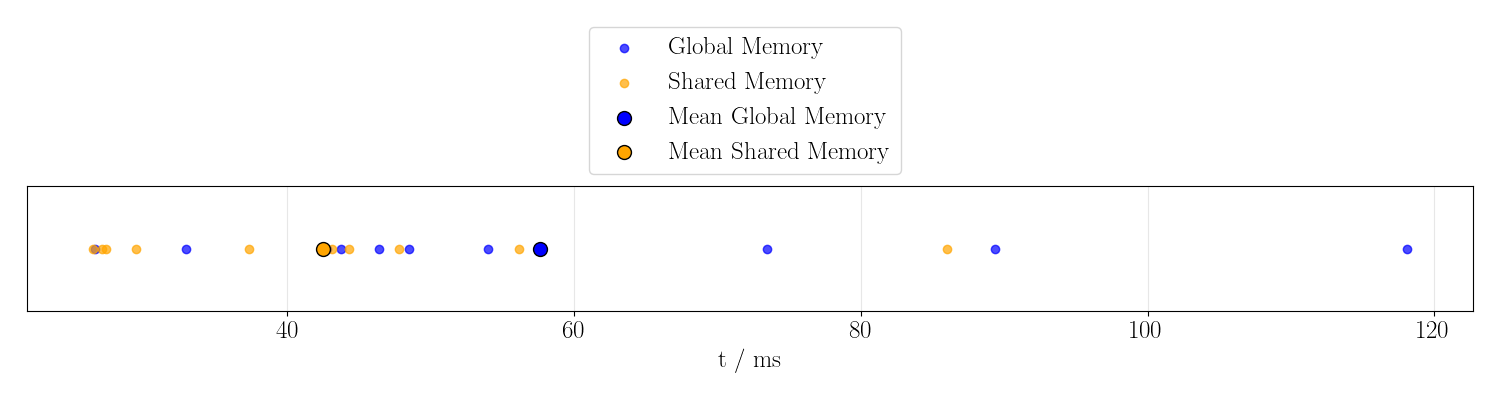
\includegraphics[width=\textwidth]{../fig/lab3/step1.png}
    \caption{Measurements }
    \label{fig:cuda_step1}
\end{figure}
Furthermore, we obtain a mean time using global memory of $t_{global} = \SI{57.6(7)}{\milli\second}$ and by using shared memory in this kernel we get $t_{shared} = \SI{42.5(3)}{\milli\second}$. 
This means we have time savings of $\SI{26(1)}{\percent}$ or about $\nicefrac{1}{4}$ when using shared memory compared to global memory. \\
\Shining{Why is shared memory faster?}\\
First and foremost we shall keep in mind, that the shared memory kernel is at a disadvantage in our comparison with the global kernel. To get insights why it still performs faster we look at benchmark results for the T4 cards to answer this question. According to a benchmark by Liu et al \footnote{Liu, Andy T., Yang, Shu-wen, Chi, Po-Han, Hsu, Pei-Hung, and Lee, Hung-yi. 
"Mockingjay: Unsupervised Speech Representation Learning with Deep Bidirectional Transformer Encoders." 
\textit{arXiv preprint arXiv:1903.07486}, 2019. \url{https://arxiv.org/abs/1903.07486}} not all cards have lower latency for shared memory compared to global memory. 

\TODO{Why faster? -> maybe data locality}
\subsection{Step 2: Execution time for different N and threads per block}
I implemented a small loop to run the GPU code for 5 different $N$ with $N \in \{50, 500, 2000, 4000, 5000\}$. The resulting time benchmarks for 32, 64 and 100 threds per block can be seen in \autoref{fig:cuda_step2}. 
\begin{figure}[H]
    \centering
    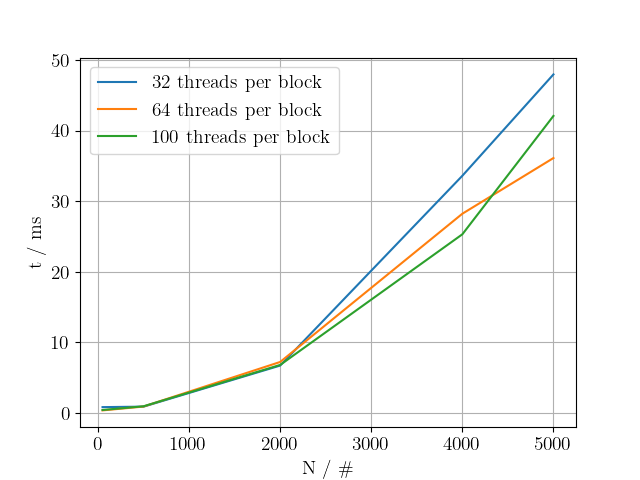
\includegraphics[width=0.5\textwidth]{../fig/lab3/step2.png}
    \caption{Runtime for $N \in \{50, 500, 2000, 4000, 5000\}$ and for 32, 64 and 100 threads per block respectively.}
    \label{fig:cuda_step2}
\end{figure}
\TODO{maybe add somethin, justification whatever?!}
\subsection{Step 3: Speedups}
We measure two different scenarios: 
\begin{enumerate}[i]
    \item excluding time of memory copy from CPU $\rightarrow$ GPU
    \item including time of memory copy from CPU $\rightarrow$ GPU
\end{enumerate}
After measuring \Shining{5} rounds without (i) and with (ii) memory access time we obtain the following \Shining{scatter plot} in \autoref{fig:cuda_step3}
\begin{figure}[H]
    \centering
    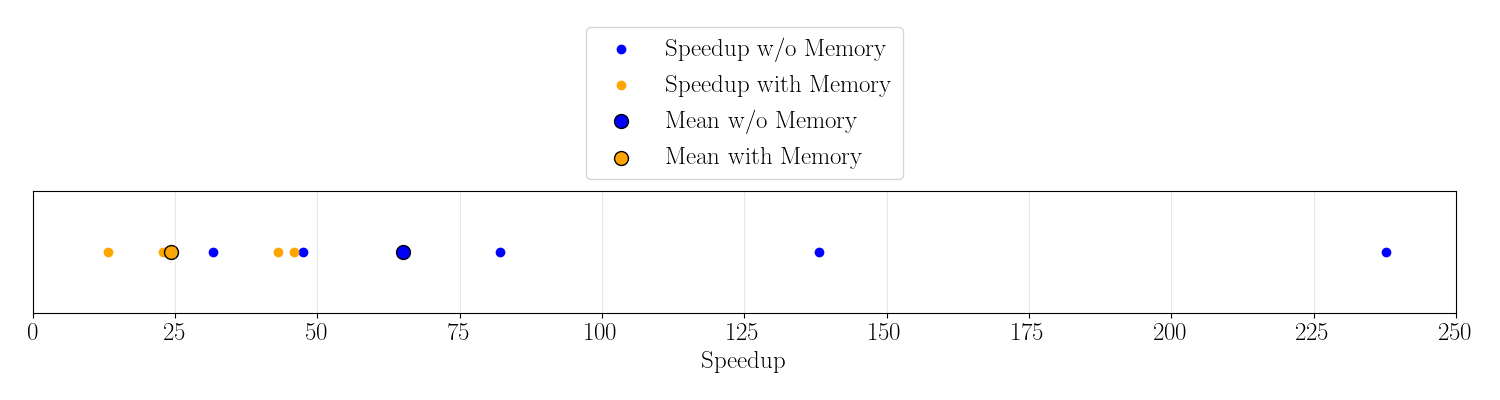
\includegraphics[width=\textwidth]{../fig/lab3/step3.png}
    \caption{Speedup of GPU implementation vs. CPU with and without memory transfer times.}
    \label{fig:cuda_step3}
\end{figure}
The mean speedup without memory access times is $\times 65$ and with memory access timed it comes out to $\times 24$.
\subsection{Step 4: Explanation of the results}
\TODO{Mach was hier Junge!!!}
